\newpage
\section{Entorno operacional}

\noindent En este apartado se explicará el software utilizado así como el robot Baxter y sus componentes. Se comenzará con ROS, el middleware que permite integrar las tareas de control, y a continuación se hablará de MoveIt! y RViz y las plataformas utilizadas para realizar la manipulación y visualización del modelo y del movimiento. \\

\subsection{ROS}

\noindent Robotic Operating System \cite{ROS} \cite{ROS2} es un framework libre orientado a desarrollo de aplicaciones para robots. Actúa como un sistema operativo incluyendo abstracción de hardware, transferencia de mensajes entre procesos, administración de paquetes, etc. Para el desarrollo de software cuenta con librerías y herramientas que permiten construir, ejecutar y escribir código en cualquier lenguaje de programación. \\
\noindent Cada versión de ROS está montada sobre un sistema basado en Unix, aunque actualmente se está integrando en otros sistemas como Windows. \\


\subsubsection{Conceptos}
\noindent En ROS existen una serie de conceptos básicos a integrar:

\begin{itemize}
	\item Paquetes. Son la unidad básica de organización de ROS y contienen los nodos, librerías y ficheros de configuración como CMakeLists.txt y package.xml. Se pueden construir a partir de la orden catkin\_create\_package, que crea automáticamente los archivos de configuración.
	\item Nodos. Son los procesos de ROS, que pueden actuar como \textit{publishers} o \textit{subscribers} para enviar o recibir datos entre ellos.
	\item Mensajes. Son las estructuras de datos con las que se comunican los nodos.
	\item Tópicos. Son la vía de transporte de los mensajes, donde estos se publican.
	\item Servicios. Son otra forma de comunicación de los nodos vía petición/respuesta. 
	\item Comandos. Son una serie de órdenes para navegar por el sistema de ficheros y modificar o mostrar tópicos y mensajes. \\
\end{itemize}


\subsection{Baxter}

\begin{figure}[H]
	\centering % si queremos la imagen centrada
	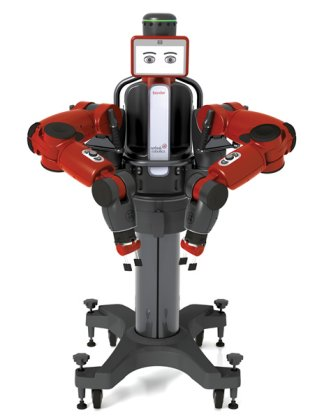
\includegraphics[scale=0.5]{imagenes/baxter1.jpg}
	\caption{Robot Baxter.}
\end{figure}

\subsubsection{Introducción}
\noindent Baxter \cite{Baxter} es un robot de automatización de procesos, desarrollado por Rethink Robotics y a la venta en el año 2012. Presenta siete grados de libertad en cada brazo y tres cámaras que se pueden utilizar o integrar en sus dos versiones disponibles: Baxter para fabricación, que incluye un entorno gráfico de fácil acceso al usuario que le permite ser programado de forma rápida y sencilla, y Baxter para investigación, para el que es necesario constar de una estación de trabajo con un entorno SDK de ROS. \\

\noindent Dos de las tres cámaras a color están situadas en los brazos y la tercera en la cabeza, donde además presenta un conjunto de sensores de ultrasonidos. Aunque consta de tres cámaras \cite{Baxter2}, sólo se pueden utilizar dos a la vez debido a las limitaciones de los USB en un entorno 64-bit.

\noindent Baxter es un robot seguro, cuenta con un botón de emergencia que deshabilita automáticamente la energía que le llega a sus componentes, de forma que cesa el proceso actual. Además consta de mecanismos de prevención de colisiones consigo mismo y, gracias a los sensores de ultrasonidos, con personas. \cite{Baxter3} \\


\subsubsection{Componentes hardware}
\label{chw}
\noindent Como se ha mencionado antes, cada brazo robótico \cite{Baxter4} tiene siete grados de libertad, lo que le permite realizar casi todos los movimientos que puede realizar un brazo humano, aunque este último conste de unos 26 grados de libertad. \\

\noindent Se utilizan actuadores elásticos que consisten en introducir un resorte entre el motor y los engranajes de las articulaciones de Baxter, proporcionando más seguridad, menos ruido de control y más estabilidad. \\

\noindent En cada brazo hay sensores infrarrojos, un acelerómetro, botones para navegar en la interfaz y, como se ha dicho anteriormente, cámaras. \\

\noindent Para nombrar cada una de las articulaciones se utilizan varias letras: S para los ``hombros'' (\textit{shoulder}), E para los ``codos'' (\textit{elbow}) y W para las ``muñecas'' (\textit{wrist}), con un número que indicará el ángulo de navegación \cite{AN}, un tipo de ángulo de Euler que se describe a continuación.

\begin{itemize}
	\item Dirección o \textit{yaw}. Rotación contraria a las agujas del reloj en el eje Z.
	\item Elevación o \textit{pitch}. Rotación contraria a las agujas del reloj en el eje Y.
	\item Ángulo de alabeo o \textit{roll}. Rotación contraria a las agujas del reloj en el eje X.
\end{itemize}

\noindent En la figura (\ref{fig:arm}) vemos cómo se denomina cada articulación de los brazos de Baxter.

\begin{figure}[H]
	\centering % si queremos la imagen centrada
	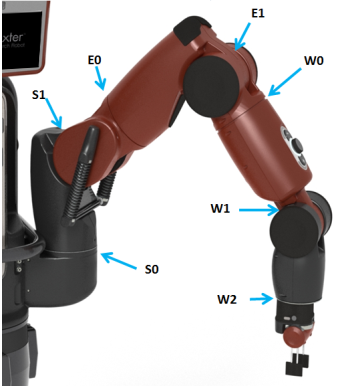
\includegraphics[scale=0.6]{imagenes/Baxter_arm.png}
	\caption{Articulaciones de Baxter.} \label{fig:arm}
\end{figure}

\noindent S0 - Shoulder Roll,
S1 - Shoulder Pitch,
E0 - Elbow Roll,
E1 - Elbow Pitch,
W0 - Wrist Roll,
W1 - Wrist Pitch,
W2 - Wrist Roll.\\

\noindent Existen dos tipos de pinzas o \textit{grippers} que se pueden colocar en los brazos de Baxter: los eléctricos y los aspiradores. Los eléctricos son dos palas paralelas que pueden levantar hasta 2 kilos aproximadamente; en cuanto a los aspiradores, se utilizan para coger objetos succionando, para lo que es necesario conectar un suministro de aire externo. \\


\subsection{MoveIt! y RViz}
\noindent MoveIt! \cite{moveit} es una plataforma de código abierto montada sobre ROS enfocada a manipulación de robots, control, cinemáticas, detección de colisiones y navegación. En este proyecto se ha utilizado para la definición de trayectorias, planificación y ejecución de las mismas, así como la detección de colisiones.\\
\noindent Para utilizar este software es necesario proporcionar el archivo URDF (es decir, el formato de modelos de robots de ROS) del robot utilizado, y MoveIt! se encarga de generar todos los archivos para comenzar a trabajar. \\
\noindent MoveIt! utiliza verificadores de colisión como FCL, una librería que detecta solapamientos entre modelos \cite{moveitfaq}. \\

\noindent El plugin RViz \cite{rviz} es una GUI de ROS (ROS Visualizer) que sirve para visualizar el modelo de robot, configurar la planificación de movimientos, evitar colisiones, además de consultar valores de los tópicos de ROS como los de las cámaras, sensores infrarrojos, etc. Normalmente se utiliza como librería de planificación la librería OMPL, de código abierto y alta calidad de planificación aleatoria. \\


\subsection{Modelos de robot}
\subsubsection{Formato universal de descripción robótica}
\noindent Este archivo URDF (\textit{Universal Robotic Description Format}), contiene la representación en formato XML del modelo de robot en estructura de árbol\cite{models2}, que, en caso de Baxter, se genera dinámicamente al iniciarlo, y actualizado cuando se conectan o desconectan los \textit{grippers} o pinzas o cuando se coge o suelta un objeto \cite{models}. Contiene información sobre la descripción cinemática o dinámica del robot, representación visual, modelo de colisión y enlaces entre las articulaciones \cite{models3} [p. 60-61]. \\


\subsubsection{Formato semántico de descripción robótica}

\noindent El archivo SRDF (\textit{Semantic Robot Description Format}) se genera dinámicamente al iniciar MoveIt! y complementa al archivo URDF. Contiene los parámetros necesarios para establecer los límites de las articulaciones de los brazos y articulaciones virtuales, información sobre cinemática y controladores y verificadores de colisión adicionales \cite{models3} [p. 122]. \\
